L'avvento e la diffusione di Internet ha rivoluzionato il mondo in cui viviamo e reso possibile tra le altre cose anche una nuova concezione di apprendimento. Nascono quindi i primi servizi di E-Learning che nel corso degli anni si sono evoluti e oggi giorno vengono comunemente chiamati anche MOOC (Massive Open Online Course).

La differenza sostanziale rispetto al passato sta nel fatto che le piattaforme MOOC offrono generalmente corsi aperti a chiunque, in cui la partecipazione è gratuita e permettono interattività tra gli studenti.

L'enorme potenziale di tali sistemi è stato compreso sin da subito e già nel 2012 tali servizi erano circa 100 e quasi 700 nel 2013, con una media di 2 nuovi MOOC al giorno.


% Il mercato globale dell'e-learning dovrebbe raggiungere 107.000 milioni di dollari entro la fine del 2015.

Secondo i dati disponibili, il giro di affari collegato all'e-learning è ingente, ma considerato l'elevato numero di piattaforme presenti, il mercato risulta molto frammentato, tuttavia, la fetta più importante è occupata dalle piattaforme principali quali Coursera, EdX, Udacity, Udemy e SkillShare.

% Secondo i dati disponibili, il giro di affari collegato all'e-learning è ingente, si stima infatti che nel 2015 il fatturato complessivo, a livello mondiale, sia stato di 107.000 milioni di dollari \cite{teleskill}. In ogni modo visto l'elevato numero di piattaforme presenti, il mercato risulta molto frammentato tuttavia una grande fetta è occupato da Coursera, EdX, Udacity, Udemy e SkillShare.

Atenei prestigiosi quali Stanford, Harvard, Berkeley e MIT utilizzano tali piattaforme per erogare parte della propria offerta formativa, estendendo cosi il loro bacino di utenza.
I corsi offerti ricoprono diverse tematiche e vengono erogati direttamente dai Professori di tali atenei universitari.

Il modello di business di tali servizi consente l'accesso gratuito cavalcando la filosofia tipica dei MOOC, viene pero richiesto un compenso nel caso in cui si desideri ottenere una certificazione, rilasciata solo dopo aver superato un test per verificare il reale livello di apprendimento.

Eliminando barriere temporali e spaziali, questi sistemi hanno il merito di diminuire la difficoltà di accesso alla formazione di livello universitario, e sono spesso invocati come contributori quando non direttamente artefici, di una vera e propria rivoluzione nel mondo dell'istruzione.

Negli ultimi tempi si è vista la diffusione di un modello alternativo a quello introdotto sinora: al posto di un ente autoritativo nel campo della formazione, quale ad esempio un prestigioso ateneo, che eroga un corso tramite uno dei propri docenti, alcune piattaforme stanno introducendo la possibilità di strutturare un corso on-line per chiunque lo ritenga opportuno.

Questo ad esempio è il caso di Udemy, che ha riscontrato subito un grande successo, ed è stato sfruttato da molte persone che, hanno pubblicato sulla piattaforma numerosi corsi, alcuni dei quali risultano accessibili previo pagamento e diventano quindi una vera e propria fonte di guadagno per il docente.

\begin{figure}[htb] %  figure placement: here, top, bottom
 \centering
 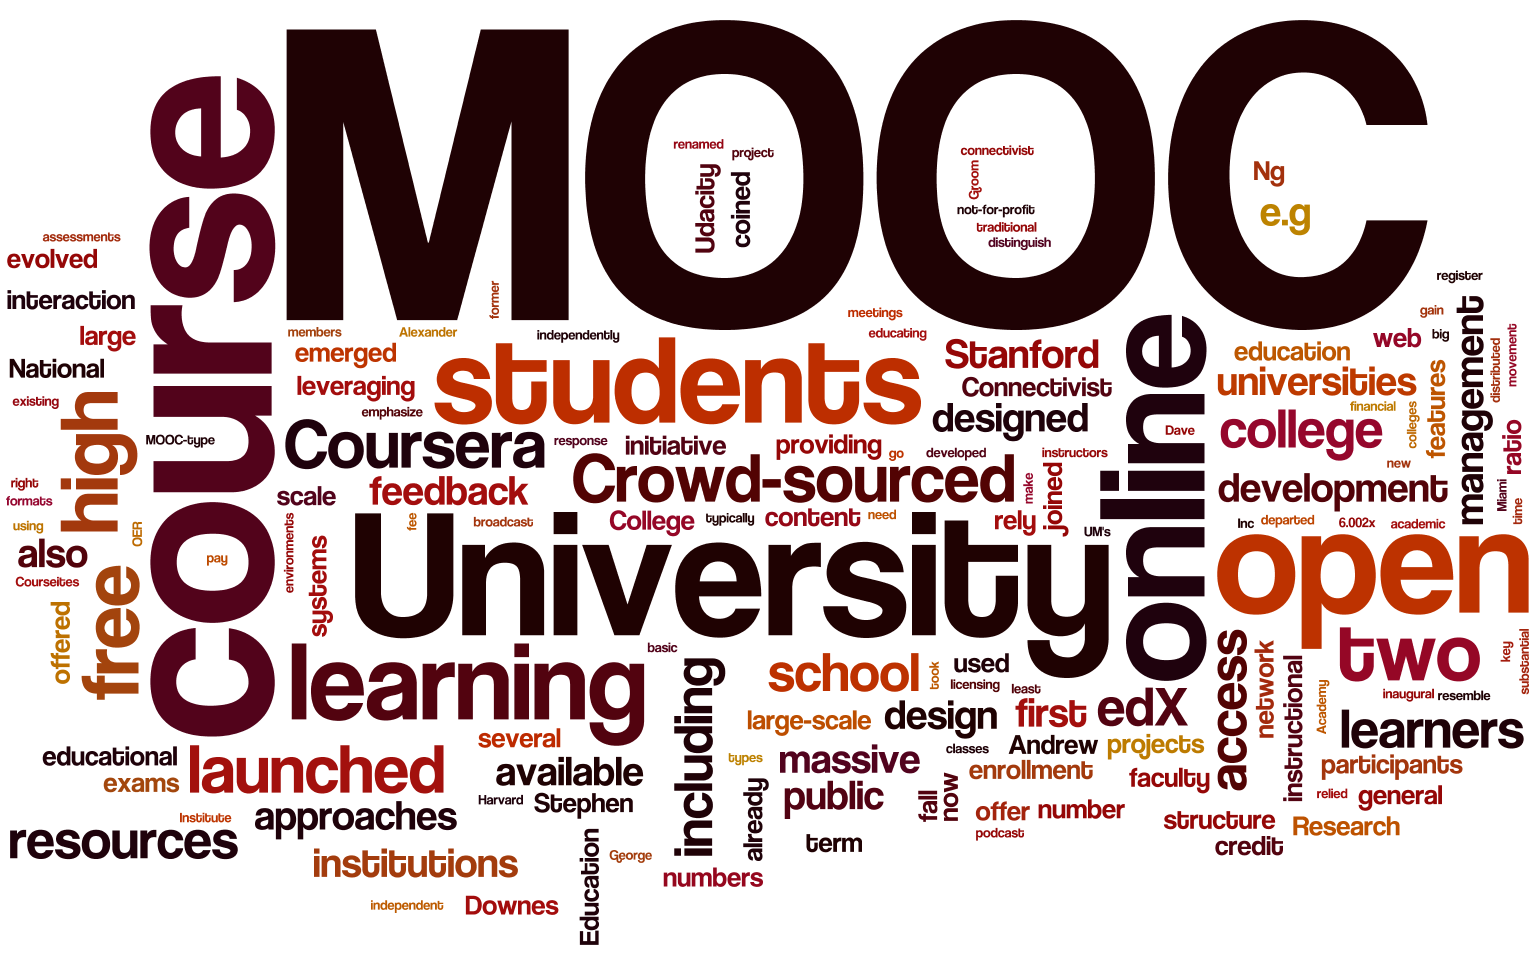
\includegraphics[width=0.7\linewidth]{images/introduction/mooc.png}\hfill
 \caption[Mooc image]{Mooc image}
 \label{fig:fourV}
\end{figure}


Nonostante l'avvento di HTML5 la gestione video rimane ancora molto insidiosa. Non esiste infatti uno standard per lo streaming video in grado di garantire la fruzione dei contenuti su i diversi web browser e dispositivi mobili.

Infatti la mancanza di protocolli condivisi dai vendor, unitamente alla enorme mole di dati che occorre gestire confrontandosi con contenuti video, individuano uno scoglio tecnologico da affrontare e superare.

La creazione di un serizio di e-learning richiede inoltre investimenti onerosi per coprire i costi di realizzazione, storage e soprattuto per il traffico dati necessario allo streaming dei contenuti video.


L'obiettivo di questo lavoro di tesi svolto presso il CVDLAB è stato quello di approfondire e astrarre le metodologie e le tecnologie utili a superare lo scoglio tecnologico individuato al fine di offrire l'opportunita a utenti e principalmente aziende di creare la propria piattaforma di E-Learning.

Un possibile fruitore della piattaforma potrebbe essere ad esempio una grande azienda che vuole creare una propria sezione Academy tramite la quale formare il personale senza dover necessariamente appogiarsi a terzi. 

Infine è stato adottato il concetto di riusabilità dei componenti tratto dallo standard HTML5 Web Components che ha facilitato notevolmente la creazione di un caso d'uso finale: X-Learning.
X-learning è una piattaforma strutturata in due parti distinte: una parte di amministrazione indirizzata all'utente che può gestire l'organico dei docenti e introdurre corsi e una parte per gli utenti che invece necessitano la fruizine dei contenuti.

La tesi si articola in due parti, ognuna delle quali consta di 3 capitoli:
Nel primo capitolo viene offerta una panoramica sulle principali piattaforme MOOC esistenti.
Il secondo capitolo invece descrive i servizi utilizzati per la realizzazione della piattaforma e una breve analisi dei costi.
Nel terzo capitolo invece vengono illustrate le tecnologie adottate per lo sviluppo.
Con l'inizio della seconda parte della tesi entriamo nel dettaglio del progetto, in particolar modo nel quarto capitolo avremo una panoramica della architettura e organizzazione della piattaforma.
Nel quinto capitolo ci focalizzeremo su componenti principali realizzati nel progetto e su come sono stati realizzati.
Il sesto e ultimo capitolo espone le conclusioni tratte e fornisce dei possibili sviluppi futuri, focalizzandosi sulle problematiche di messa in produzione, non affrontate direttamente durante il lavoro di tesi.